\chapter{Энтропия чёрных дыр, голография и пространство де Ситтера}

\lectureoverview{Мы завершаем аргумент соответствия, начатый на предыдущей лекции. Сильно возбуждённая струна обладает энтропией, пропорциональной её массе, тогда как шварцшильдовская чёрная дыра обладает энтропией, пропорциональной её площади. Эти две формулы связаны не отождествлением сильно гравитирующей чёрной дыры со свободной струной, а медленным изменением струнной константы связи до тех пор, пока эти два описания не встретятся. Затем закон площади естественным образом приводит к голографическому принципу, а в заключительной части лекции вводятся расширяющееся пространство и геометрия де Ситтера, горизонт которой будет изучаться далее.}

\section{Возвращение к задаче подсчёта}

В подсчёте для длинной струны оставалась одна недоговорённость. Если фиксированная полная длина распределена между несколькими струнами, то одинаковые струны одной и той же длины неразличимы. Тем не менее их положения в ящике входят в состояние, а сам ящик выбирается примерно того размера, который занимает соответствующая одиночная длинная струна.

\begin{classroomqa}
\audiencequestion{Различаются ли короткие струны между собой, и учитываются ли их положения?\lecturetimestamp{00:00:37}}
\lecturerresponse{Струны с одинаковыми свойствами неразличимы, но их положения в ящике учитываются. Сравнение проводится при фиксированном объёме, выбранном так, чтобы он совпадал с областью, занимаемой длинной струной.}
\end{classroomqa}

После этого можно сформулировать цель. Мы соберём короткий список уравнений и используем его, чтобы получить масштабное поведение энтропии чёрной дыры. Не потребуется ни интеграл, ни бесконечная сумма. Трудность не алгебраическая; она состоит в том, чтобы знать, какие величины можно сравнивать и на каком этапе рассуждения.

\section{Натуральные единицы и планковская площадь}

Положим
\begin{equation}
c=\hbar=1,
\label{eq:l07-natural-units}
\end{equation}
но оставим ньютоновскую постоянную в явном виде. Первое следствие состоит в том, что время и длина имеют одинаковые размерности. Соотношение для фотона
\begin{equation}
E=\frac{\hbar c}{\lambda}
\end{equation}
и соотношение массы и энергии \(E=mc^2\) тогда дают
\begin{equation}
[M]=L^{-1}.
\label{eq:l07-mass-dimension}
\end{equation}
Следовательно, массу можно выражать как обратную длину.

\begin{figure}[htbp]
\centering
\includegraphics[width=0.62\textwidth]{lecture_07_figure_02.png}
\caption{Соглашение о натуральных единицах в начале рассуждения о размерностях. Формула для энергии дополняется уравнениями, приведёнными выше.}
\lectureframe{00:03:27.900}
\end{figure}

Чтобы определить размерность \(G_N\), используем ньютоновское ускорение только как средство учёта размерностей:
\begin{equation}
a\sim\frac{G_NM}{R^2}.
\end{equation}
Поскольку \(T\) и \(L\) имеют одинаковую размерность, \([a]=L/T^2=L^{-1}\). Вместе с уравнением~\eqref{eq:l07-mass-dimension} это даёт
\begin{equation}
[G_N]=L^2.
\end{equation}
В этих единицах ньютоновская постоянная имеет размерность площади. Определяя планковскую длину как
\begin{equation}
G_N=\ell_p^2,
\label{eq:l07-planck-area}
\end{equation}
мы сразу понимаем, почему \(A/G_N=A/\ell_p^2\) безразмерно: оно измеряет площадь в единицах планковской площади.

\section{Струнная константа связи и сила гравитации}

Теперь гравитацию нужно перевести на язык струн. Полезная картина — это процесс обмена. Когда струна самопересекается, она может расщепиться и вновь соединиться. Маленькая петля замкнутой струны может быть испущена одним объектом и поглощена другим; когда это возбуждение является гравитоном, процесс опосредует гравитацию. Один множитель взаимодействия возникает при испускании, а другой — при поглощении, так что сила обмена содержит \(g_s^2\).

Константа связи \(g_s\) безразмерна. Точнее, это константа связи на уровне амплитуды, тогда как вероятность или скорость процесса начинается с порядка \(g_s^2\).\editorialnote{В лекции \(g_s\) иногда называется вероятностью, а затем это исправляется на квадратный корень из вероятности. Пертурбативная константа связи относится к уровню амплитуды.} Поскольку \(G_N\) имеет размерность площади, всё ещё не хватает масштаба длины. Его даёт фундаментальная струнная длина \(\ell_s\), масштаб одного элементарного колебания струны:
\begin{equation}
G_N\sim g_s^2\ell_s^2,
\qquad
\ell_p\sim g_s\ell_s.
\label{eq:l07-planck-string}
\end{equation}

\begin{figure}[htbp]
\centering
\includegraphics[width=0.72\textwidth]{lecture_07_figure_05.png}
\caption{Соотношение для константы связи на доске: \(G_N=\ell_p^2\) и \(g_s^2\ell_s^2\sim\ell_p^2\).}
\lectureframe{00:12:15.000}
\end{figure}

При слабой связи, \(g_s\ll1\), планковская длина намного меньше струнной длины. Уменьшение \(g_s\) ослабляет гравитацию, оставляя элементарный струнный масштаб фиксированным.\editorialnote{Для эффективной четырёхмерной теории в \(G_N\) также входят данные компактификации и численные соглашения. В этом рассуждении о масштабах они считаются фиксированными и опускаются.}

\section{Подсчёт для длинной струны}

Энтропия подсчитывает элементарные выборы, необходимые для задания состояния. Заменим сильно возбуждённую струну блужданием по квадратной решётке. В каждой вершине следующее звено может быть направлено в одну из четырёх сторон. Описывать элементарный выбор как один выбор из четырёх возможностей или как два бинарных выбора меняет лишь константу порядка единицы. Существенно число шагов.

Если \(L\) — контурная длина струны, а каждый шаг имеет длину \(\ell_s\), то требуется
\begin{equation}
N=\frac{L}{\ell_s}
\end{equation}
шагов. Число блужданий растёт экспоненциально, схематически как \(\Omega_N\sim q^N\), где \(q\) имеет порядок единицы, и потому
\begin{equation}
S_{\mathrm{str}}=\log\Omega_N\sim N\sim\frac{L}{\ell_s}.
\label{eq:l07-string-entropy-length}
\end{equation}

\begin{figure}[htbp]
\centering
\includegraphics[width=0.68\textwidth]{lecture_07_figure_03.png}

\vspace{0.7em}
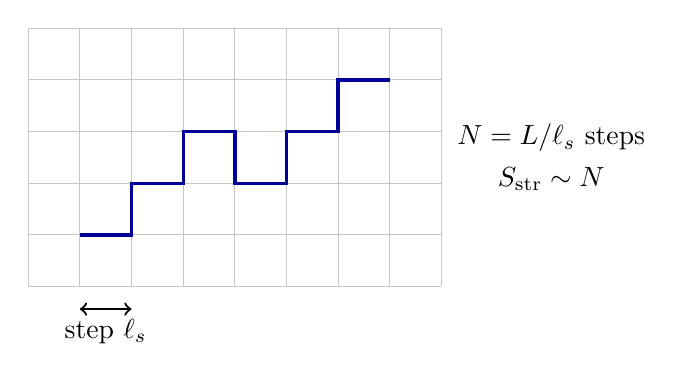
\begin{tikzpicture}[scale=0.82]
  \draw[step=0.8cm,gray!45,thin] (0,0) grid (6.4,4.0);
  \draw[very thick,blue!60!black]
    (0.8,0.8)--(1.6,0.8)--(1.6,1.6)--(2.4,1.6)--(2.4,2.4)--
    (3.2,2.4)--(3.2,1.6)--(4.0,1.6)--(4.0,2.4)--(4.8,2.4)--
    (4.8,3.2)--(5.6,3.2);
  \draw[<->,thick] (0.8,-0.35)--(1.6,-0.35);
  \node[below] at (1.2,-0.35) {step \(\ell_s\)};
  \node[align=center] at (8.1,2.0) {\(N=L/\ell_s\) steps\\[0.3em]\(S_{\mathrm{str}}\sim N\)};
\end{tikzpicture}
\caption{Решёточная модель на доске и её приведённая в порядок интерпретация как случайного блуждания. Число выборов определяется контурной длиной, а не диаметром спутанного клубка.}
\lectureframe{00:17:20.000}
\end{figure}

Масса также подсчитывается по тем же элементарным сегментам. Сегмент длины \(\ell_s\) имеет масштаб массы
\begin{equation}
m_{\mathrm{seg}}\sim\frac{1}{\ell_s}.
\end{equation}

\begin{classroomqa}
\audiencequestion{Элементарному сегменту приписывается длина \(\ell_s\)?\lecturetimestamp{00:18:56}}
\lecturerresponse{Да. Его характерная длина равна \(\ell_s\), поэтому в натуральных единицах его характерная масса равна \(1/\ell_s\).}
\end{classroomqa}

Складывая массы \(L/\ell_s\) сегментов, получаем
\begin{equation}
M\sim\frac{L}{\ell_s}\frac{1}{\ell_s}
=\frac{L}{\ell_s^2},
\qquad
L\sim M\ell_s^2.
\label{eq:l07-string-mass}
\end{equation}
Кинетическая и потенциальная энергии колеблющейся струны здесь сжаты в это масштабное соотношение; более подробное статистико-механическое рассмотрение даёт ту же зависимость. Подстановка в уравнение~\eqref{eq:l07-string-entropy-length} приводит к формуле для струны, которая нам понадобится:
\begin{equation}
S_{\mathrm{str}}\sim M\ell_s.
\label{eq:l07-string-entropy-mass}
\end{equation}

\begin{figure}[htbp]
\centering
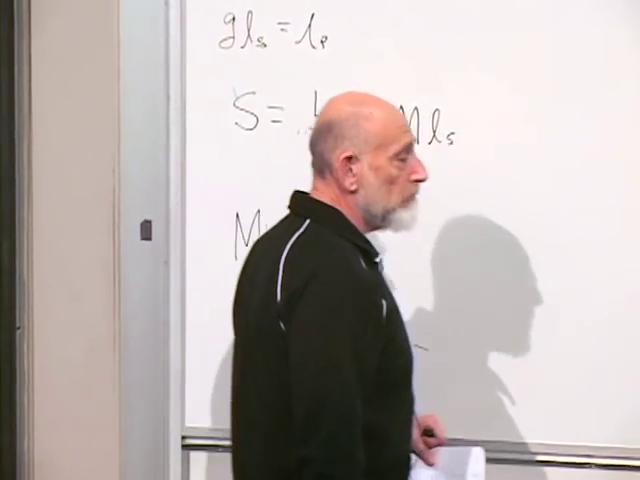
\includegraphics[width=0.66\textwidth]{lecture_07_figure_04.png}
\caption{Столбец со струнной стороны, собранный перед сравнением: \(\ell_p\sim g_s\ell_s\), \(S_{\mathrm{str}}\sim L/\ell_s\sim M\ell_s\) и \(M\sim L/\ell_s^2\).}
\lectureframe{00:21:57.800}
\end{figure}

\section{Почему свободная струна — это ещё не чёрная дыра}

Со стороны гравитации точная полуклассическая формула имеет вид
\begin{equation}
S_{\mathrm{BH}}=\frac{A}{4G_N}.
\label{eq:l07-bh-exact}
\end{equation}

\begin{classroomqa}
\audiencequestion{Какой численный коэффициент должен стоять в знаменателе?\lecturetimestamp{00:23:28}}
\lecturerresponse{Четыре. Аргумент соответствия восстановит масштабную зависимость, но он слишком груб, чтобы определить этот точный множитель.}
\end{classroomqa}

Для четырёхмерной шварцшильдовской чёрной дыры
\begin{equation}
R_s=2G_NM,
\qquad
A=4\pi R_s^2.
\end{equation}
Если, как в лекции, опустить численные множители,
\begin{align}
S_{\mathrm{BH}}
&\sim\frac{A}{G_N}
\sim\frac{(G_NM)^2}{G_N} \\
&\sim M^2G_N
\sim M^2\ell_p^2.
\label{eq:l07-bh-scaling}
\end{align}

\begin{figure}[htbp]
\centering
\includegraphics[width=0.72\textwidth]{lecture_07_figure_06.png}
\caption{Завершённое сравнение на доске: струнная энтропия — это длина в струнных единицах, тогда как энтропия чёрной дыры — площадь в планковских единицах.}
\lectureframe{00:25:35.000}
\end{figure}

Сходство между уравнениями~\eqref{eq:l07-string-entropy-mass} и \eqref{eq:l07-bh-scaling} наводит на мысль о связи, но это не одна и та же формула. Было бы неверно просто назвать исходную чёрную дыру свободной струной и выполнить подстановку. Подсчёт для свободной струны не учитывает притяжение между частями струны — именно то взаимодействие, которое сжимает её в чёрную дыру и понижает её полную энергию за счёт отрицательной энергии связи.

Ошибка хорошо знакома по примеру звезды. Горячий газ звёздной массы, помещённый в слишком большой ящик, не является моделью звезды, даже при той же температуре. Самогравитация изменяет равновесный размер и связь между энергией и энтропией. Отслеживать каждое самовзаимодействие длинной струны было бы трудно, поэтому мы не будем этого делать.

\begin{classroomqa}
\audiencequestion{Если от длинной струны отделяется маленькая петля, её энтропия уменьшается. Означает ли это, что обмен гравитонами понижает энтропию гравитирующей системы?\lecturetimestamp{00:28:48}}
\lecturerresponse{Нет, не в том равновесном обменном процессе, который используется здесь. Виртуальные возбуждения испускаются и поглощаются в обоих направлениях; эта схема не означает буквальную потерю постоянного фрагмента струны. Единственная цель этой схемы здесь — установить два множителя связи и, следовательно, зависимость от \(g_s^2\).}
\end{classroomqa}

\section{Адиабатическая игра соответствия}

Вместо этого начнём там, где гравитацией можно пренебречь. При \(g_s\to0\) струны пересекаются, не расщепляясь и не соединяясь, и самогравитационное притяжение исчезает. Увеличивайте \(g_s\), удерживая \(\ell_s\) фиксированным: гравитация усиливается, сильно возбуждённая струна сжимается и в конце концов становится чёрной дырой. Медленно поверните этот параметр обратно, и чёрная дыра должна вернуться в струнное состояние. Она может перейти в небольшое число длинных струн, но подсчёт состояний при высоких энергиях из предыдущей лекции говорит, что доминирующий сектор содержит одну длинную струну, а не огромный газ из коротких.

\begin{classroomqa}
\audiencequestion{Что удерживается фиксированным при изменении константы связи?\lecturetimestamp{00:32:19}}
\lecturerresponse{Фиксированной удерживается струнная длина \(\ell_s\), а значит и элементарный струнный масштаб массы \(1/\ell_s\). Регулятор изменяет \(g_s\) и, следовательно, \(G_N\sim g_s^2\ell_s^2\).}
\end{classroomqa}

Изменение должно быть медленным, изолированным и обратимым. При этих условиях энтропия является адиабатическим инвариантом:
\begin{equation}
\Delta S=0.
\label{eq:l07-adiabatic}
\end{equation}
Одной лишь медленности недостаточно, если происходят диссипативные или неконтролируемые переходы. Здесь ``адиабатический'' означает, что одно и то же семейство состояний можно непрерывно прослеживать.\editorialnote{Это термодинамический смысл адиабатичности, связанный с обратимыми процессами. Необратимый процесс может быть адиабатическим в смысле отсутствия теплопередачи и всё же производить энтропию.}

Пусть рассматриваемая чёрная дыра имеет массу \(M_0\) и константу связи \(g_{s,0}\). До использования формулы площади, которую мы пытаемся объяснить, анализ размерностей говорит лишь, что энтропия нейтральной невращающейся чёрной дыры является некоторой функцией безразмерной комбинации
\begin{equation}
S_{\mathrm{BH}}=f(M\ell_p)
=f(Mg_s\ell_s).
\label{eq:l07-entropy-function}
\end{equation}
При фиксированной \(\ell_s\) изоэнтропический путь, следовательно, сохраняет
\begin{equation}
Mg_s=M_0g_{s,0}
\label{eq:l07-adiabat}
\end{equation}
постоянной, при условии что прослеживается одна и та же ветвь состояний.

По мере уменьшения \(g_s\) отрицательная энергия связи устраняется, так что масса \(M\) вдоль этого пути возрастает. Соответствующая струнная конфигурация тоже становится менее тесно связанной и расплывается. Однако формальный радиус Шварцшильда на адиабате ведёт себя как \(R_s\sim Mg_s^2\ell_s^2\sim g_s\ell_s\) и потому уменьшается.\editorialnote{В устном обсуждении к объекту, освобождаемому от гравитационной связи, применяется слово ``растёт''. Это не следует понимать так, будто радиус Шварцшильда вдоль выведенной адиабаты увеличивается.}

\begin{classroomqa}
\audiencequestion{Увеличивается объект или уменьшается по мере ослабления гравитации?\lecturetimestamp{00:36:28}}
\lecturerresponse{Его струнная структура высвобождается и расширяется, тогда как масса увеличивается, поскольку отрицательная энергия связи устраняется. Радиус, приписываемый формулой чёрной дыры, уменьшается, пока не достигает струнного масштаба, где такое описание в терминах чёрной дыры перестаёт быть полезным.}
\end{classroomqa}

\section{Две кривые и их пересечение}

Отложим массу по вертикали, а струнную константу связи — по горизонтали. Уравнение ~\eqref{eq:l07-adiabat} задаёт гиперболу, \(M\propto g_s^{-1}\).

\begin{classroomqa}
\audiencequestion{Какой вид имеет кривая с постоянным произведением \(Mg_s\)?\lecturetimestamp{00:44:08}}
\lecturerresponse{Гипербола. Это адиабата, проходящая через рассматриваемую точку \((g_{s,0},M_0)\).}
\end{classroomqa}

Вторая кривая отмечает кроссовер между описаниями. Чёрную дыру уже нельзя разрешить как обычную геометрию Шварцшильда, когда её радиус меньше элементарного колебания струны. Поэтому точку соответствия мы оцениваем из условия
\begin{equation}
R_s\sim\ell_s.
\label{eq:l07-correspondence-radius}
\end{equation}
Используя \(R_s\sim MG_N\) и уравнение ~\eqref{eq:l07-planck-string}, получаем
\begin{equation}
Mg_s^2\ell_s^2\sim\ell_s,
\qquad
Mg_s^2\sim\frac{1}{\ell_s}.
\label{eq:l07-transition-curve}
\end{equation}
Таким образом, кривая перехода убывает как \(M\propto g_s^{-2}\), круче, чем адиабата.

\begin{figure}[htbp]
\centering
\includegraphics[width=0.70\textwidth]{lecture_07_figure_07.png}

\vspace{0.6em}
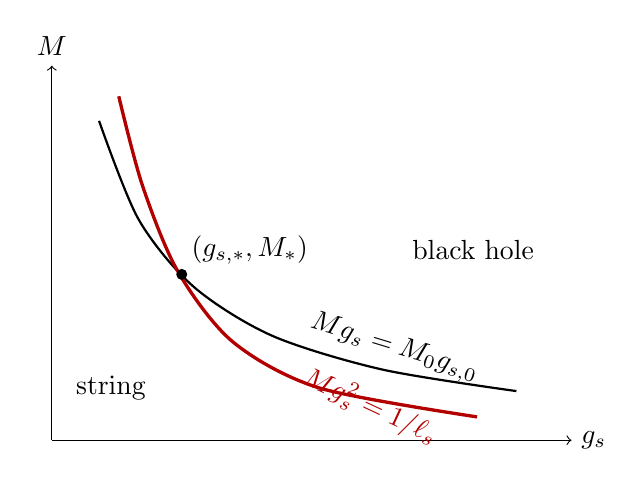
\begin{tikzpicture}[x=1cm,y=0.78cm]
  \draw[->] (0.4,0.4)--(7.0,0.4) node[right] {\(g_s\)};
  \draw[->] (0.4,0.4)--(0.4,6.5) node[above] {\(M\)};
  \draw[thick,black] plot[smooth] coordinates {(1.0,5.6) (1.5,4.0) (2.2,2.9) (3.2,2.1) (4.6,1.55) (6.3,1.2)};
  \draw[very thick,red!70!black] plot[smooth] coordinates {(1.25,6.0) (1.55,4.55) (2.0,3.15) (2.7,2.0) (3.8,1.25) (5.8,0.78)};
  \fill (2.05,3.1) circle (2pt) node[above right] {\((g_{s,*},M_*)\)};
  \node[black,rotate=-17] at (4.75,1.9) {\(Mg_s=M_0g_{s,0}\)};
  \node[red!70!black,rotate=-25] at (4.45,0.95) {\(Mg_s^2=1/\ell_s\)};
  \node at (5.75,3.5) {black hole};
  \node at (1.15,1.25) {string};
\end{tikzpicture}
\caption{График с доски и его аккуратная интерпретация. Чёрная адиабата пересекает более крутую красную кривую соответствия в точке, где объект становится струноподобным.}
\lectureframe{00:49:35.000}
\end{figure}

В точке пересечения \((M_*,g_{s,*})\) два уравнения имеют вид
\begin{align}
M_*g_{s,*} &= M_0g_{s,0}, \\
M_*g_{s,*}^2 &\sim \frac{1}{\ell_s}.
\end{align}
Возведём первое уравнение в квадрат и разделим на второе:
\begin{equation}
M_*
\sim M_0^2g_{s,0}^2\ell_s.
\end{equation}
Умножая на \(\ell_s\),
\begin{equation}
M_*\ell_s
\sim M_0^2g_{s,0}^2\ell_s^2
\sim M_0^2G_{N,0}.
\label{eq:l07-crossover-result}
\end{equation}

\begin{figure}[htbp]
\centering
\includegraphics[width=0.68\textwidth]{lecture_07_figure_08.png}
\caption{Завершённая алгебра перехода, включая \(M_*\ell_s=M_0^2g_{s,0}^2\ell_s^2=M_0^2G_{N,0}\).}
\lectureframe{00:54:40.000}
\end{figure}

\begin{classroomqa}
\audiencequestion{После деления уравнений двух кривых \(\ell_s\) должно оказаться в числителе или в знаменателе?\lecturetimestamp{00:52:41}}
\lecturerresponse{В числителе. Деление на \(1/\ell_s\) равносильно умножению на \(\ell_s\), поэтому \(M_*\sim M_0^2g_{s,0}^2\ell_s\).}
\end{classroomqa}

В точке перехода применима струнная формула, так что
\begin{equation}
S_*\sim M_*\ell_s.
\end{equation}
Энтропия вдоль пути не изменялась. Сочетая это утверждение с уравнением ~\eqref{eq:l07-crossover-result}, получаем энтропию исходной чёрной дыры:
\begin{equation}
S_{\mathrm{BH}}(M_0)
\sim M_0^2G_{N,0}
\sim M_0^2\ell_{p,0}^2.
\label{eq:l07-final-correspondence}
\end{equation}
Это и есть искомое масштабирование по закону площади.

\section{Что соответствие доказывает и чего не доказывает}

Эта конструкция не утверждает, что исходная, сильно гравитирующая чёрная дыра является свободной струной. Она переводит объект в режим, где подсчёт струнных состояний надёжен, считывает там энтропию и переносит её обратно вдоль обратимого пути. Переход является кроссовером, а не резко локализованной фазовой границей, поэтому эта оценка не может определить коэффициент \(1/4\) в уравнении ~\eqref{eq:l07-bh-exact}.

Тем не менее та же логика работает на уровне параметрических оценок для заряженных чёрных дыр, чёрных объектов в других размерностях и протяжённых чёрных бран. Более симметричные и суперсимметричные примеры допускают защищённые подсчёты состояний, сохраняющие точную информацию при изменении константы связи; эти методы восстанавливают численные коэффициенты, но вводят математический аппарат, не нужный для настоящего концептуального аргумента.

Наиболее важно то, что это вычисление даёт микроскопическую интерпретацию. Энтропия служит свидетельством скрытой структуры. Гидродинамика описывает плотность, давление и течение, не упоминая молекулы; энтропия жидкости показывает, что такие микроскопические степени свободы существуют. Общая теория относительности аналогично описывает горизонт, не показывая его микросостояния. Подсчёт струнных состояний показывает, что непротиворечивая квантовая теория гравитации может содержать достаточно состояний, чтобы объяснить энтропию чёрной дыры.

\begin{classroomqa}
\audiencequestion{Что означало бы \(S\sim M^3\ell_p^3\) вместо квадратичного результата?\lecturetimestamp{00:59:41}}
\lecturerresponse{Это выглядело бы как закон объёма. Обычное вещество в комнате или чашке кофе имеет энтропию, пропорциональную объёму; квадратичный ответ особенный, потому что через \(R_s\sim M\ell_p^2\) он пропорционален площади горизонта.}
\end{classroomqa}

Этот результат свидетельствует о том, что энтропия Бекенштейна--Хокинга — не просто формальная термодинамическая аналогия. Он указывает на микроскопические гравитационные степени свободы, хотя элементарный вывод не делает эти степени свободы видимыми по отдельности.

\section{От максимальной энтропии к голографии}

Теперь мы меняем вопрос. Вместо того чтобы спрашивать об энтропии заданного состояния, спросим о наибольшей энтропии, совместимой с данной областью.

Начнём с обычной решёточной модели комнаты. Разобьём объём на ячейки размера \(V_{\mathrm{cell}}\), и пусть каждой ячейке соответствует один вопрос с ответом да или нет: занята или пуста. Сасскинд даёт воображаемому атому нарочито нелепое название ``мясоний'', чтобы никакие реалистические атомные детали не отвлекали от подсчёта. Если
\begin{equation}
N=\frac{V}{V_{\mathrm{cell}}},
\end{equation}
то число конфигураций и максимальная энтропия равны
\begin{equation}
\Omega=2^N,
\qquad
S_{\max}=\log\Omega=N\log2
\sim\frac{V}{V_{\mathrm{cell}}}.
\label{eq:l07-volume-count}
\end{equation}

\begin{figure}[htbp]
\centering
\includegraphics[width=0.68\textwidth]{lecture_07_figure_09.png}
\caption{Комната, разделённая на ячейки, с двумя состояниями на ячейку. Здесь подсчитывается максимальная энтропия, а не энтропия упорядоченной комнаты, занятой слушателями.}
\lectureframe{01:05:20.000}
\end{figure}

Реальная комната намного ниже этого максимума. Состояние, которое хаотически исследовало бы все эти варианты заполнения ячеек, было бы чрезвычайно горячим. От игрушечной модели сохраняется обычное ожидание, что число независимых степеней свободы, а следовательно и максимальная энтропия, масштабируются с объёмом.

Гравитация опровергает это ожидание. Рассмотрим сферическую область с площадью границы \(A\), начальной энтропией \(S_{\mathrm{i}}\) и массой \(M\), меньшей, чем масса \(M_{\mathrm{BH}}\) чёрной дыры, которая как раз заполнила бы сферу. Если бы \(M\) было больше, горизонт уже выходил бы за выбранную границу.

Теперь отправим внутрь оболочку массой \(M_{\mathrm{BH}}-M\). Её состав несущественен; в лекции допускаются свет, обычное вещество или даже швейцарский сыр. Устроим так, чтобы она сколлапсировала. Конечное состояние — чёрная дыра, горизонт которой как раз заполняет область, с энтропией
\begin{equation}
S_{\mathrm{f}}=\frac{A}{4G_N}.
\end{equation}
Второй закон требует
\begin{equation}
S_{\mathrm{i}}\le S_{\mathrm{f}}
=\frac{A}{4G_N}.
\label{eq:l07-holographic-bound}
\end{equation}

\begin{figure}[htbp]
\centering
\includegraphics[width=0.70\textwidth]{lecture_07_figure_10.png}

\vspace{0.5em}
\begin{tikzpicture}[scale=0.88]
  \draw[thick] (0,0) circle (1.35);
  \draw[very thick,red!70!black] (0,0) circle (2.05);
  \fill[gray!25] (0,0) circle (1.32);
  \node at (0,0) {\(M,S_{\mathrm{i}}\)};
  \draw[-{Latex[length=3mm]},thick,red!70!black] (3.5,0)--(2.15,0);
  \node[align=center,right] at (3.5,0) {incoming shell\\\(M_{\mathrm{BH}}-M\)};
  \node[below] at (0,-2.2) {final horizon area \(A\)};
\end{tikzpicture}
\caption{Конструкция с оболочкой. Внутрь посылается достаточно дополнительной массы, чтобы образовалась чёрная дыра, горизонт которой как раз заполняет выбранную область.}
\lectureframe{01:13:30.000}
\end{figure}

Поскольку чёрная дыра такого размера является допустимым состоянием и насыщает это неравенство, максимальная энтропия равна
\begin{equation}
S_{\max}=\frac{A}{4G_N}.
\label{eq:l07-holographic-maximum}
\end{equation}
Это и есть голографический принцип в его счётной формулировке: максимальное число независимых степеней свободы в гравитирующей области масштабируется с площадью её границы, приблизительно по одной степени свободы порядка единицы на каждую планковскую площадь, а не с числом заключённых внутри планковских объёмов.\editorialnote{Аргумент с оболочкой предполагает, что область можно охватить и заставить сколлапсировать указанным образом. Для более общих пространств-времён требуются ковариантные энтропийные ограничения, но сферический аргумент передаёт принцип, используемый в лекции.}

Несоответствие огромно. Интуиция локальной теории поля подсказывает, что выборы, сделанные в разных внутренних точках, должны комбинироваться независимо, давая закон объёма. Гравитация говорит, что достаточно большое число таких выборов само бы сколлапсировало, и чёрная дыра даёт большую допустимую энтропию. Поэтому граничный подсчёт — не малая поправка к объёмному; это иная организация гильбертова пространства.

\begin{classroomqa}
\audiencequestion{Что происходит для очень большой Вселенной с примерно однородной плотностью?\lecturetimestamp{01:15:48}}
\lecturerresponse{Этот вопрос требует космологии, а не статической сферической конструкции. Именно он мотивирует немедленный переход к расширяющимся решениям уравнений Эйнштейна.}
\end{classroomqa}

\begin{classroomqa}
\audiencequestion{Связано ли ограничение по площади с принципом неопределённости?\lecturetimestamp{01:16:03}}
\lecturerresponse{Лекция оставляет этот вопрос открытым и затем переходит к космологии.}
\end{classroomqa}

\section{Расширяющееся пространство}

Мы не будем здесь выводить космологические решения из уравнений Эйнштейна; мы просто запишем решения и научимся их читать. Пространственные срезы могут быть положительно искривлёнными и замкнутыми, отрицательно искривлёнными и гиперболическими или плоскими. В дальнейшем обсуждении возьмём пространственно-плоские евклидовы срезы в нестационарном пространстве-времени.

\begin{classroomqa}
\audiencequestion{Каков пространственно-временной аналог обычного евклидова пространства?\lecturetimestamp{01:19:37}}
\lecturerresponse{Пространство Минковского. Рассматриваемая здесь космологическая модель имеет плоские пространственные срезы, но не является пространством-временем Минковского, поскольку её пространственная метрика меняется со временем.}
\end{classroomqa}

Знакомая картинка с воздушным шаром описывает замкнутую расширяющуюся поверхность размерностью на единицу меньше. Susskind вспоминает, как пытался провести эту демонстрацию с большим размеченным шаром; маркер ослабил резину и привёл к буквальному хлопку. Этот случай также обнаруживает концептуальный изъян аналогии. Когда обычный шарик расширяется, молекулы резины расходятся, и материал истончается, пока не рвётся. В космологическом пространстве локальные законы не размываются. Чтобы сохранить аналогию, нужно воображать, что всё новые молекулы резины непрерывно вставляются, так что каждый малый участок сохраняет одни и те же локальные свойства. В плоской модели замените шарик большим листом, который равномерно растягивают наружу и так же пополняют новым материалом.

Математически расширение входит в метрику:
\begin{equation}
\begin{aligned}
ds^2&=-dt^2+a(t)^2d\mathbf{x}^2,\\
d\mathbf{x}^2&=\delta_{ij}\,dx^i dx^j
=dx^2+dy^2+dz^2.
\end{aligned}
\label{eq:l07-frw-metric}
\end{equation}

\begin{figure}[htbp]
\centering
\includegraphics[width=0.72\textwidth]{lecture_07_figure_11.png}
\caption{Пространственно-плоская расширяющаяся метрика, записанная на доске.}
\lectureframe{01:25:10.000}
\end{figure}

Точки, сохраняющие фиксированные пространственные координаты, называются сопутствующими. Если две такие точки имеют координатное расстояние \(\Delta x\), то их собственное расстояние в момент \(t\) равно
\begin{equation}
D(t)=a(t)\Delta x.
\label{eq:l07-proper-distance}
\end{equation}
Их координаты не меняются, но метрическое расстояние между ними меняется. Дифференцируя при фиксированном \(\Delta x\),
\begin{equation}
V=\dot D=\dot a\,\Delta x
=\frac{\dot a}{a}D.
\end{equation}
Введём параметр Хаббла
\begin{equation}
H(t)=\frac{\dot a(t)}{a(t)}.
\label{eq:l07-hubble-parameter}
\end{equation}
Тогда
\begin{equation}
V=H(t)D,
\label{eq:l07-hubble-law}
\end{equation}
что и есть закон Хаббла при фиксированном космическом времени.

\begin{figure}[htbp]
\centering
\includegraphics[width=0.68\textwidth]{lecture_07_figure_12.png}
\caption{Записанный на доске закон удаления при фиксированном времени: \(V=D\,\dot a/a\).}
\lectureframe{01:29:10.000}
\end{figure}

Название ``постоянная Хаббла'' может вводить в заблуждение. Вообще говоря, \(H(t)\) меняется со временем. Пространственно постоянным является отношение \(V/D\) для любой пары сопутствующих точек на одном и том же временном срезе.

\begin{classroomqa}
\audiencequestion{Для далёких галактик чьё время входит в это соотношение? Мы наблюдаем их на более ранней эпохе.\lecturetimestamp{01:31:10}}
\lecturerresponse{Уравнение~\eqref{eq:l07-hubble-law} относится к одновременному срезу. Наблюдение идёт вдоль направленного в прошлое светового луча и фиксирует далёкую галактику в более ранний момент, поэтому связь между измеренным красным смещением и расстоянием требует всей истории вдоль светового конуса, а не одного мгновенного значения \(H\).}
\end{classroomqa}

\begin{figure}[htbp]
\centering
\includegraphics[width=0.66\textwidth]{lecture_07_figure_13.png}
\caption{Пространственно-временной рисунок, используемый, чтобы отличить расстояние на срезе равного времени от того, что наблюдатель видит вдоль направленного в прошлое светового луча.}
\lectureframe{01:33:20.000}
\end{figure}

\section{Масштаб Хаббла и расширение де Ситтера}

В единицах \(c=1\) уравнение~\eqref{eq:l07-hubble-law} даёт скорость удаления, равную единице, на расстоянии
\begin{equation}
D_H=\frac{1}{H}.
\label{eq:l07-hubble-radius}
\end{equation}
Более удалённые сопутствующие точки могут иметь \(V>1\) или даже \(V\gg1\), не нарушая специальную теорию относительности. Они не пролетают мимо локального наблюдателя быстрее света; их собственное расстояние растёт, потому что расширяется геометрия между ними.\editorialnote{В общей зависящей от времени космологии \(1/H\) — это радиус Хаббла, а не автоматически горизонт событий. Он становится постоянным масштабом горизонта в случае де Ситтера, обсуждаемом далее.}

Во многих старых замедляющихся космологических моделях \(H(t)\) уменьшается, а \(1/H(t)\) растёт, так что области, когда-то удалявшиеся сверхсветово, позднее могут войти в причинный контакт. Напротив, обсуждаемая в лекции картина на поздних временах стремится к положительной постоянной \(H\). Тогда \(1/H\) остаётся фиксированным, и уравнение расширения принимает вид
\begin{equation}
\frac{\dot a}{a}=H,
\qquad
\dot a=Ha.
\label{eq:l07-constant-h}
\end{equation}

\begin{classroomqa}
\audiencequestion{Каковы единицы измерения постоянного параметра Хаббла?\lecturetimestamp{01:38:24}}
\lecturerresponse{Обратное время. Эквивалентно, при \(c=1\) это обратная длина. Величина \(H^{-1}\) задаёт и время расширения, и масштаб расстояния; в лекции приводится пример порядка величины — около пятнадцати миллиардов лет.}
\end{classroomqa}

Решение уравнения~\eqref{eq:l07-constant-h} имеет вид
\begin{equation}
a(t)=a_0e^{Ht}.
\label{eq:l07-desitter-scale-factor}
\end{equation}

\begin{classroomqa}
\audiencequestion{Какая функция имеет скорость изменения, пропорциональную самой себе?\lecturetimestamp{01:39:04}}
\lecturerresponse{Экспонента. Следовательно, масштабный фактор равен \(a_0e^{Ht}\), тогда как пространственный коэффициент \(a(t)^2\) в метрике растёт как \(e^{2Ht}\).}
\end{classroomqa}

\begin{figure}[htbp]
\centering
\includegraphics[width=0.70\textwidth]{lecture_07_figure_14.png}
\caption{Уравнения при постоянном \(H\) и их экспоненциальное решение на доске.}
\lectureframe{01:39:30.000}
\end{figure}

Пространство-время с таким экспоненциальным расширением — это пространство де Ситтера. Его постоянный масштаб Хаббла задаёт горизонт событий на конечном собственном расстоянии. Эта геометрия в некотором смысле дополняет картину чёрной дыры: наблюдатель остаётся внутри космологического горизонта, тогда как достаточно далёкие объекты удаляются и уже никогда не смогут послать сигналы, которые достигнут его. Горизонт чёрной дыры скрывает внутреннюю область от внешнего наблюдателя; горизонт де Ситтера скрывает внешнюю часть области, доступной наблюдателю. В отличие от обычной испаряющейся чёрной дыры, идеальная геометрия де Ситтера рассматривается здесь как сохраняющаяся во времени. Здесь это сравнение только начинается. В следующей лекции подробнее рассматриваются горизонт, его термодинамика и загадки, которые он создаёт для космологии.
